% ==============================================================================
% WEEK 3
% ==============================================================================
\section{Week 3 -- 02.03.26 - Complex Integration}
\textit{(Chapter 10 in the book)}

\begin{recall}[Recall: Vector Analysis]
If $\vec{F}$ is a continuous vector field on $\R^2$, so $\vec{F} : \R^2 \rightarrow \R^2$, it can be written as $\vec{F}(x_1, x_2) = (F_1(x_1, x_2), F_2(x_1, x_2))$. 

Let $\gamma : [a,b] \longrightarrow \R^2$ be a $C^1$ curve with image $\Gamma$. The line integral is defined by:
\[
\int_{\Gamma} \vec{F} \cdot d\vec{l} := \int_a^b \vec{F}(\gamma(t)) \cdot \gamma'(t) \, dt
\]
Orientation will be important! The inner product is given by:
\[
F_1(\gamma(t)) \cdot \gamma_1'(t) + F_2(\gamma(t)) \cdot \gamma_2'(t)
\]
\textbf{Key points:}
\begin{itemize}
    \item The integral is \textbf{independent of the parametrization}.
    \item If we \textbf{switch orientation}, the integral has the opposite sign.
    \item If the curve is \textbf{closed} (i.e., $\gamma(a) = \gamma(b)$) and the curl is zero ($\curl \vec{F} = 0$) in the interior of $\Gamma$, then $\int_{\Gamma} \vec{F} \cdot d\vec{l} = 0$.
    \item A curve is \textbf{simple} if there are no self-intersections.
    \item A curve is \textbf{regular} if $\gamma'(t) \neq 0$.
\end{itemize}
\end{recall}

We will define similarly the integral of complex functions $f : \C \simeq \R^2 \longrightarrow \C \simeq \R^2$.

\begin{definition}[Definition]
Let $\gamma : [a,b] \rightarrow \C$ be a regular curve that parametrizes $\Gamma$. \\
Let $f : \C \rightarrow \C$ be a continuous function. Then the complex integral is defined by:
\[
\int_{\Gamma} f(z) \, dz = \int_{\gamma} f(z) \, dz := \int_a^b f(\gamma(t)) \cdot \gamma'(t) \, dt
\]
\textit{(Note: this involves complex multiplication!)}

\vspace{0.2cm}
\textbf{Usual notation:} The integral over the curve with the opposite orientation (often denoted $-\Gamma$) has the opposite sign:
\[
\int_{-\Gamma} f(z) \, dz = - \int_{\Gamma} f(z) \, dz
\]
\end{definition}

\noindent The value of the integral is independent of the parametrization, as long as the orientation is the same.

\begin{example}[Example 1]
Let $\Gamma$ be the unit half-circle around $z=0$, parametrized counter-clockwise.

\begin{center}
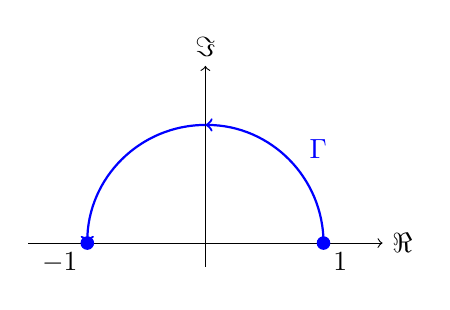
\begin{tikzpicture}[scale=1.5]
    \draw[->] (-1.5,0) -- (1.5,0) node[right] {$\Re$};
    \draw[->] (0,-0.2) -- (0,1.5) node[above] {$\Im$};
    \draw[thick, blue, ->] (1,0) arc (0:90:1);
    \draw[thick, blue, ->] (0,1) arc (90:180:1);
    \node[blue, right] at (0.8, 0.8) {$\Gamma$};
    \filldraw[blue] (1,0) circle (1.5pt) node[black, below right] {$1$};
    \filldraw[blue] (-1,0) circle (1.5pt) node[black, below left] {$-1$};
\end{tikzpicture}
\end{center}

Parametrization: $\gamma : [0, \pi] \rightarrow \C, \quad \gamma(t) = e^{it}$. \\
Derivative: $\gamma'(t) = i e^{it}$. \\
Integrate $f(z) = z^2$ over $\Gamma$:
\begin{align*}
\int_{\Gamma} z^2 \, dz &= \int_0^\pi (e^{it})^2 \cdot i e^{it} \, dt \\
&= i \int_0^\pi e^{3it} \, dt \\
&= i \left[ \frac{e^{3it}}{3i} \right]_{t=0}^{t=\pi} = \frac{e^{3i\pi} - e^0}{3} = \frac{-1 - 1}{3} = \mathbf{-\frac{2}{3}}
\end{align*}
\textit{Note: We used the fundamental theorem of calculus and the fact that $e^{\lambda t} = \frac{1}{\lambda} (e^{\lambda t})'$ for $\lambda \in \C$. For more general functions, we can always split into real and imaginary parts and compute the two (real) integrals separately.}
\end{example}

\begin{example}[Example 2]
Let $\Gamma = \{ z : |z| = 1 \}$ counter-clockwise (full circle). \\
$\gamma(t) = e^{it}$ for $t \in [0, 2\pi]$, and $\gamma'(t) = ie^{it}$.
\begin{align*}
\int_{\Gamma} z^2 \, dz &= \int_0^{2\pi} (e^{it})^2 i e^{it} \, dt \\
&= i \int_0^{2\pi} e^{3it} \, dt = i \left[ \frac{e^{3it}}{3i} \right]_0^{2\pi} = \frac{1 - 1}{3} = \mathbf{0}
\end{align*}
\textit{Observation: Integrals of holomorphic functions are governed by similar rules as integrals of vector fields with curl = 0.}
\end{example}

\begin{example}[Examples 3 and 4]
With the same $\Gamma$ (counter-clockwise unit circle):
\begin{itemize}
    \item For $f(z) = \frac{1}{z}$:
    \[ \int_{\Gamma} \frac{1}{z} \, dz = \int_0^{2\pi} \frac{1}{e^{it}} i e^{it} \, dt = i \int_0^{2\pi} 1 \, dt = \mathbf{2\pi i \neq 0} \]
    \item For $f(z) = \frac{1}{z^2}$:
    \[ \int_{\Gamma} \frac{1}{z^2} \, dz = \int_0^{2\pi} \frac{1}{(e^{it})^2} i e^{it} \, dt = i \int_0^{2\pi} e^{-it} \, dt = i \left[ \frac{e^{-it}}{-i} \right]_0^{2\pi} = -(1 - 1) = \mathbf{0} \]
\end{itemize}
\end{example}

\subsection{Cauchy's Theorem}

\begin{theorem}[Theorem]
Let $U$ be an open and \textbf{simply connected} set, and let $\Gamma$ be a closed and piecewise regular curve inside $U$. \\
If $f : U \rightarrow \C$ is \textbf{holomorphic}, then:
\[
\int_{\Gamma} f(z) \, dz = 0
\]
\end{theorem}

\textbf{Remarks:}
\begin{enumerate}
    \item \textbf{Simply connected:} Means it has only one component and has no "holes".
    \begin{itemize}
        \item $\C$: Simply connected.
        \item $\{z : |z| < 1\}$ (Disk): Simply connected.
        \item $\C \setminus \{0\}$: \textbf{NOT} simply connected.
    \end{itemize}
    \item \textbf{In practice:} We are given $f$ and $\Gamma$, and we try to find a simply connected set $U$ which contains $\Gamma$ and lies inside the domain where $f$ is holomorphic.
\end{enumerate}

\begin{proofbox}[Proof (Outline)]
Let $\gamma(t) = \alpha(t) + i\beta(t)$ be the parametrization, and $f(x+iy) = u(x,y) + i v(x,y)$.
\begin{align*}
\int_{\Gamma} f(z) \, dz &= \int_a^b f(\gamma(t)) \cdot \gamma'(t) \, dt \\
&= \int_a^b \Big(u(\gamma(t)) + i v(\gamma(t))\Big) \Big(\alpha'(t) + i\beta'(t)\Big) \, dt \\
&= \underbrace{\int_a^b (u \alpha' - v \beta') \, dt}_{\text{Real part}} + i \underbrace{\int_a^b (v \alpha' + u \beta') \, dt}_{\text{Imaginary part}}
\end{align*}

We can rewrite this as the integral of two real vector fields. Let $\vec{F} = (u, -v)$ and $\vec{G} = (v, u)$. The equation becomes:
\[
= \int_{\Gamma} \vec{F} \cdot d\vec{l} + i \int_{\Gamma} \vec{G} \cdot d\vec{l}
\]
Since $U$ is simply connected and $\Gamma \subseteq U$, the interior of $\Gamma$ (denoted $\text{int}(\Gamma)$) is entirely contained in $U$. $\vec{F}$ and $\vec{G}$ are well defined on $\text{int}(\Gamma)$. Applying \textbf{Green's theorem}:
\[
= \iint_{\text{int}(\Gamma)} \curl \vec{F} \, dxdy + i \iint_{\text{int}(\Gamma)} \curl \vec{G} \, dxdy
\]
Now, let's calculate the curls:
\begin{itemize}
    \item $\curl \vec{F} = \partial_x(-v) - \partial_y(u) = -v_x - u_y$
    \item $\curl \vec{G} = \partial_x(u) - \partial_y(v) = u_x - v_y$
\end{itemize}
By the \textbf{Cauchy-Riemann equations} (since $f$ is holomorphic, we have $u_x = v_y$ and $u_y = -v_x$). So $\curl \vec{F} = 0$ and $\curl \vec{G} = 0$.
The integral is therefore $0 + i0 = 0$.
\end{proofbox}

\begin{example}[Examples]
\begin{itemize}
    \item For $\Gamma = \{z : |z| = 1\}$ and $f(z) = z^2$. Applying Cauchy's theorem for $U=\C$: $\int_{\Gamma} z^2 \, dz = 0$.
    \item For the same $\Gamma$ and $f(z) = \frac{1}{z}$. $f$ is holomorphic on $\C \setminus \{0\}$. There is \textbf{no} simply connected set $U \subseteq \C \setminus \{0\}$ which contains $\Gamma$ (because $\Gamma$ surrounds the "hole" at $0$). Cauchy's theorem does not apply (and we saw earlier that the integral is $2\pi i \neq 0$).
\end{itemize}
\end{example}

\begin{example}[Example: Shifted circle]
Let $f(z) = \frac{1}{z}$ and $\Gamma = \{ z : |z - 2| = 1 \}$.\\
If we choose $U = \{ z : \Re(z) > 0 \}$ (the right half-plane), it is simply connected, $f$ is holomorphic there, and $\Gamma \subset U$. So by Cauchy's theorem: $\int_{\Gamma} \frac{1}{z} \, dz = \mathbf{0}$.

\textbf{Explicit verification:} $\gamma(t) = 2 + e^{it}, \quad \gamma'(t) = i e^{it}$.
\begin{align*}
\int_{\Gamma} f(z) \, dz &= \int_0^{2\pi} \frac{1}{2 + e^{it}} \cdot i e^{it} \, dt \\
&= \int_0^{2\pi} \frac{d}{dt} \Big(\log(2 + e^{it})\Big) \, dt \\
&= \Big[ \log(2 + e^{it}) \Big]_0^{2\pi} = \mathbf{0}
\end{align*}
\textit{Explanation: We use the fact that the argument of $\log$ does not go through the negative real line along the curve, so $\log(z)$ remains differentiable with $(\log z)' = 1/z$.}
\end{example}

\subsection{An Extension of Cauchy's Theorem (Deformation)}

\begin{theorem}[Theorem: Contour Deformation]
Let $\Gamma_0, \Gamma_1$ be closed, simple, regular curves with $\Gamma_1 \subset \text{int}(\Gamma_0)$ (one is inside the other). Let $\gamma_0, \gamma_1$ be parametrizations of $\Gamma_0, \Gamma_1$ with the \textbf{same orientation}.

If $f$ is holomorphic on the region \textbf{between} the curves (i.e. on $\text{int}(\Gamma_0) \setminus \text{int}(\Gamma_1)$), then:
\[
\int_{\Gamma_0} f(z) \, dz = \int_{\Gamma_1} f(z) \, dz
\]
\end{theorem}

\begin{proofbox}[Proof (Idea)]
Consider two new closed paths (say $C_0$ and $C_1$) by connecting $\Gamma_0$ and $\Gamma_1$ with line segments (a "cut"). Since $f$ is holomorphic in the interior of both complete paths without holes, the integral over each is $0$.
By adding the two together, the integrals over the segments cover the same path with opposite orientations and cancel out. We are left with the integral over $\Gamma_0$ in the correct direction, and the integral over $\Gamma_1$ in the opposite direction. Hence the result.
\end{proofbox}

\textbf{Usefulness:} Very useful result. It can be used to "shift" the curve of integration and obtain a simpler integral.

\begin{example}[Example: The Square]
Compute $\int_{\Gamma} \frac{1}{z} \, dz$ where $\Gamma$ is the square with vertices $2+2i, -2+2i, -2-2i, 2-2i$, oriented counter-clockwise.

Since $f(z) = 1/z$ is holomorphic on $\C \setminus \{0\}$, we can deform this square into the unit circle $\Gamma_1 = \{ z : |z| = 1 \}$. The origin $0$ is a problem, but it is located inside both curves, so the area "between the square and the circle" is perfectly safe and holomorphic.
\[
\int_{\text{Square}} \frac{1}{z} \, dz = \int_{|z|=1} \frac{1}{z} \, dz = \mathbf{2\pi i}
\]
(The same value we computed earlier!).
\end{example}

\subsection{Cauchy Integral Formulas}

\begin{theorem}[Theorem: Cauchy Formula]
Suppose that $D \subseteq \C$ is open and $f : D \rightarrow \C$ is holomorphic. If $z_0 \in D$, then:
\[
f(z_0) = \frac{1}{2\pi i} \int_{\gamma} \frac{f(z)}{z - z_0} \, dz
\]
for any closed, simple curve $\gamma$ inside $D$ which contains $z_0$ in its interior and is oriented counter-clockwise.
\end{theorem}

\begin{proofbox}[Proof (Idea)]
The function defined by $z \mapsto \frac{f(z)}{z - z_0}$ is holomorphic in $D \setminus \{z_0\}$.
By applying the extension of Cauchy's theorem, we can deform $\gamma$ into a very small circle $\gamma_1$ around $z_0$ of radius $r > 0$.
Parametrization: $\gamma_1(t) = z_0 + r e^{it}$ for $t \in [0, 2\pi]$.
\begin{align*}
\int_{\gamma} \frac{f(z)}{z - z_0} \, dz &= \int_{\gamma_1} \frac{f(z)}{z - z_0} \, dz \\
&= \int_0^{2\pi} \frac{f(z_0 + r e^{it})}{r e^{it}} \cdot \Big( i r e^{it} \Big) \, dt \\
&= i \int_0^{2\pi} f(z_0 + r e^{it}) \, dt
\end{align*}
Now, we let the radius approach zero ($r \rightarrow 0$). Since $f$ is continuous at $z_0$, the integral becomes:
\[
\lim_{r \to 0} i \int_0^{2\pi} f(z_0 + r e^{it}) \, dt = i \int_0^{2\pi} f(z_0) \, dt = i \cdot f(z_0) \cdot 2\pi = \mathbf{2\pi i f(z_0)}
\]
Dividing by $2\pi i$, we obtain the formula.
\end{proofbox}